% ============================================================
%  Truck-N-Trailer Autonomous Parking System — ME 235 Report
%  Compile with pdflatex (Overleaf compatible, TeX Live 2023+)
% ============================================================
\documentclass[11pt, letterpaper]{article}

% --- Layout ---
\usepackage[margin=1in]{geometry}
\usepackage[T1]{fontenc}
\usepackage[utf8]{inputenc}
\usepackage{lmodern}
\usepackage{microtype}

% --- Math ---
\usepackage{amsmath, amssymb}

% --- Graphics & figures ---
\usepackage{graphicx}
\usepackage{float}
\usepackage{caption}

% --- TikZ for architecture diagram ---
\usepackage{tikz}
\usetikzlibrary{positioning, shapes.geometric, arrows.meta,
                fit, backgrounds, calc}

% --- Code listings ---
\usepackage{listings}
\usepackage{xcolor}

\definecolor{codebg}{rgb}{0.97,0.97,0.97}
\definecolor{codekw}{rgb}{0.10,0.10,0.65}
\definecolor{codecomment}{rgb}{0.40,0.40,0.40}
\definecolor{codestr}{rgb}{0.15,0.50,0.15}

\lstset{
  backgroundcolor=\color{codebg},
  basicstyle=\ttfamily\small,
  keywordstyle=\color{codekw}\bfseries,
  commentstyle=\color{codecomment}\itshape,
  stringstyle=\color{codestr},
  breaklines=true,
  breakatwhitespace=true,
  frame=single,
  framesep=4pt,
  rulecolor=\color{black!20},
  numbers=none,
  tabsize=2,
  showstringspaces=false,
  columns=flexible,
}
\lstdefinestyle{clang}{language=C,
  morekeywords={uint8_t, int8_t, BaseType_t, TaskHandle_t,
                gptimer_handle_t, gptimer_alarm_event_data_t,
                IRAM_ATTR, pdFALSE, pdTRUE, EncoderState}}
\lstdefinestyle{python}{language=Python,
  morekeywords={self, pyo, Any}}

% --- Tables ---
\usepackage{booktabs}

% --- Hyperlinks ---
\usepackage{hyperref}
\hypersetup{
  colorlinks=true,
  linkcolor=blue!60!black,
  citecolor=blue!60!black,
  urlcolor=blue!60!black,
}

% --- Spacing ---
\usepackage{parskip}
\setlength{\parskip}{7pt plus 2pt minus 1pt}

% --- Section formatting ---
\usepackage{titlesec}
\titleformat{\section}{\large\bfseries}{}{0em}{\thesection\quad}
\titleformat{\subsection}{\normalsize\bfseries}{\thesubsection}{1em}{}
\titlespacing{\section}{0pt}{14pt}{6pt}
\titlespacing{\subsection}{0pt}{10pt}{4pt}

% ============================================================
\begin{document}

% ---- Title page --------------------------------------------------------
\begin{titlepage}
  \centering
  \vspace*{3.5cm}
  {\Huge\bfseries Truck-N-Trailer Autonomous Parking System\par}
  \vspace{1.2cm}
  {\large ME 235 Final Project Report\par}
  \vspace{1.8cm}
  {\normalsize
    Eric Chuang \enspace$\bullet$\enspace
    Evan Grealish \enspace$\bullet$\enspace
    Aryan Kulkarni \enspace$\bullet$\enspace
    Xiao Liu\par}
  \vspace{0.6cm}
  {\normalsize May 12, 2026\par}
\end{titlepage}

% ---- 1. Background and Motivation -------------------------------------
\section{Background and Motivation}

Backing up a truck with a trailer is one of the most challenging things
to do behind the wheel. It is a nonholonomic problem and you must ensure
the system does not jackknife. It takes experienced drivers years to
develop the skills for this control action. Because of this, it is an
interesting control problem that is explored in this project.

This project builds a small physical model of the truck and trailer
system with motors controlled by an ESP32 board, and integrates overhead
vision and a laptop-hosted route planning stack. Our goal is to simulate
a real-world situation where a driver needs to park a truck and trailer
system, and could navigate into place manually or with an auto parking
feature.

% ---- 2. GUI, Real-Time, and Multitasking ------------------------------
\section{Description of GUI, Real-Time, and Multitasking Implementation}

\subsection{Graphical User Interface}

The interface is organized around two main modes:

\begin{itemize}
  \item \textbf{Manual Mode:} Provides forward, back, left, and right
    control buttons. A speed slider lets the user set the target RPM,
    and the GUI sends wheel commands directly over UART to the ESP32.

  \item \textbf{Automatic Mode:} Engages the MPC controller. A
    Start/Stop button initiates the autonomous parking sequence. The GUI
    feeds the current state from computer vision into the planner, then
    sends the resulting wheel speed commands to the firmware.
\end{itemize}

As shown in Figure~\ref{fig:gui}, the GUI also displays a live overhead
camera view drawn via OpenCV, including bounding boxes for the truck and
trailer, the defined parking spot, and the planned trajectory from the
MPC in Automatic Mode. A simulated dial widget shows the current hitch
angle: the left dial is pulled from the potentiometer reading off the
ESP32, and the right dial is computed from the ArUco marker positions
detected by the camera. Telemetry cards show actual wheel RPMs,
commanded speeds, and connection status in real time.

Before autonomous operation can begin, the potentiometer must be
calibrated to map raw ADC counts to physical hitch angle in degrees. The
GUI provides a step-by-step calibration wizard: the user positions the
hitch at four known angles (maximum negative, zero, maximum positive,
and zero again to capture hysteresis), captures a measurement at each
step, and the system fits a piecewise-linear mapping. This calibration
is a prerequisite for accurate hitch-angle feedback in both the
dashboard display and the MPC state estimator.

\begin{figure}[H]
  \centering
  % -------------------------------------------------------------------
  % Replace the placeholder below with the actual screenshot:
  %   \includegraphics[width=\textwidth]{gui_screenshot.png}
  % Upload gui_screenshot.png to Overleaf alongside this file.
  % -------------------------------------------------------------------
  \fbox{\parbox{0.92\textwidth}{\centering\vspace{2.2cm}
    \textit{[Insert GUI screenshot here — upload
    \texttt{gui\_screenshot.png} to Overleaf]}
    \vspace{2.2cm}}}
  \caption{GUI of Truck-n-Trailer (Automatic Mode, MPC running).}
  \label{fig:gui}
\end{figure}

% ---- 2.2 Real-Time ----------------------------------------------------
\subsection{Real-Time Implementation}

Real-time behavior in this system spans two computing layers with
different timing requirements and different notions of ``real-time.''

\paragraph{Firmware --- hard real-time.}
The ESP32 runs motor PID control at a fixed 100\,Hz loop rate. This is
hard real-time: the PID algorithm requires a consistent $\Delta t$ to
produce stable control output, and the GPTimer ISR enforces this with
hardware-level precision independent of task scheduling. Encoder
telemetry (motor RPMs and potentiometer reading) is sent to the laptop
at 10\,Hz. The 100\,Hz rate was chosen to be fast enough to track
velocity targets accurately across the full RPM range while leaving
sufficient headroom for the lower-priority communication task.

\paragraph{Laptop --- soft real-time.}
The laptop side runs two \texttt{QTimer} callbacks within a single
PyQt6 event loop:

\begin{itemize}
  \item \textbf{Camera timer (30\,Hz, 33\,ms interval):} Each tick
    grabs a frame from the overhead camera
    (\texttt{cv2.VideoCapture.read()}, blocking I/O) then runs ArUco
    marker detection (\texttt{detectMarkers()}, typically 10--25\,ms
    depending on frame content and marker visibility). When three
    markers are found (truck~ID~0, trailer~ID~1, goal~ID~10), the
    pipeline computes world-frame poses and outputs the vehicle state
    vector \texttt{vision\_q} and goal position \texttt{goal\_xy}.
    Effective throughput is therefore 10--30\,fps in practice.

  \item \textbf{Send timer (10\,Hz, 100\,ms interval):} Polls the UART
    receive buffer for the latest telemetry, runs the MPC solver if in
    autonomous mode, and writes the resulting RPM targets back over
    UART. The MPC solve is the dominant cost in this callback: IPOPT
    typically converges in 50--200\,ms with a warm start from the
    previous solution. Because this runs synchronously in the Qt event
    loop, a slow solve stretches the 100\,ms send interval, introducing
    jitter in the motor commands. The system tolerates occasional late
    commands without failure, but tracking quality degrades --- a
    soft real-time constraint.
\end{itemize}

All data and command communication between the laptop and firmware
occurs over UART at 115\,200 baud.

\begin{table}[H]
  \centering
  \caption{Timing summary across system layers.}
  \label{tab:timing}
  \begin{tabular}{llll}
    \toprule
    \textbf{Component} & \textbf{Rate} & \textbf{Deadline type}
      & \textbf{Dominant cost} \\
    \midrule
    ESP32 PID loop      & 100\,Hz & Hard  & GPTimer ISR latency ($<$1\,\textmu s) \\
    ESP32 telemetry TX  & 10\,Hz  & Soft  & UART byte write ($\sim$1\,ms) \\
    Laptop camera tick  & 30\,Hz  & Soft  & ArUco detection (10--25\,ms) \\
    Laptop send tick    & 10\,Hz  & Soft  & MPC solve (50--200\,ms) \\
    \bottomrule
  \end{tabular}
\end{table}

% ---- 2.3 Multitasking -------------------------------------------------
\subsection{Multitasking Architecture}

\paragraph{Firmware --- FreeRTOS.}
The firmware runs two concurrent FreeRTOS tasks with different
priorities:

\begin{itemize}
  \item \textbf{Control Task (higher priority):} Triggered at 100\,Hz
    by the GPTimer ISR via \texttt{vTaskNotifyGiveFromISR}. Reads
    encoder deltas, converts counts to RPM, runs independent PID
    controllers for the left and right wheels, applies a static
    feedforward term, and writes PWM outputs to the motors. Also handles
    the kill-switch state and sends telemetry at 10\,Hz.

  \item \textbf{Communication Task (lower priority):} Triggered by the
    UART receive interrupt when a full command packet arrives. Parses
    incoming target RPM values and writes them to shared state protected
    by a FreeRTOS mutex. Also reads the potentiometer ADC value and
    forwards it to the laptop in the telemetry stream.
\end{itemize}

The shared state between the two tasks is protected through FreeRTOS
synchronization primitives. If the command is stale beyond a
configurable timeout --- indicating the laptop has stopped sending --- the
Control Task automatically falls back to zero RPM as a safety measure.

The interrupt structure includes: (1)~hardware interrupts on four
encoder channels (Channel~A and B for each motor) to count quadrature
encoder pulses; (2)~an interrupt for the emergency stop button that
bypasses the normal control loop immediately; and (3)~the GPTimer alarm
ISR that unblocks the Control Task at exactly 100\,Hz.

\paragraph{Laptop --- Qt event loop.}
The laptop side uses a deliberate single-threaded design. Both timers
(camera at 30\,Hz and send at 10\,Hz) are dispatched sequentially by
the Qt event loop --- they never execute concurrently. This means the
shared vision state variables (\texttt{vision\_q}, \texttt{goal\_xy})
can be read by the send callback without locks, because the camera
callback cannot interrupt it. The tradeoff is that a blocking MPC solve
prevents the camera callback from firing until it finishes, potentially
dropping camera frames during long solves. This was an acceptable
tradeoff given the project scope; a production system would move the MPC
solve to a background thread.

\paragraph{System architecture diagram.}
Figure~\ref{fig:arch} shows the complete data-flow architecture across
both layers.

% ---- Architecture diagram ---------------------------------------------
\begin{figure}[H]
\centering
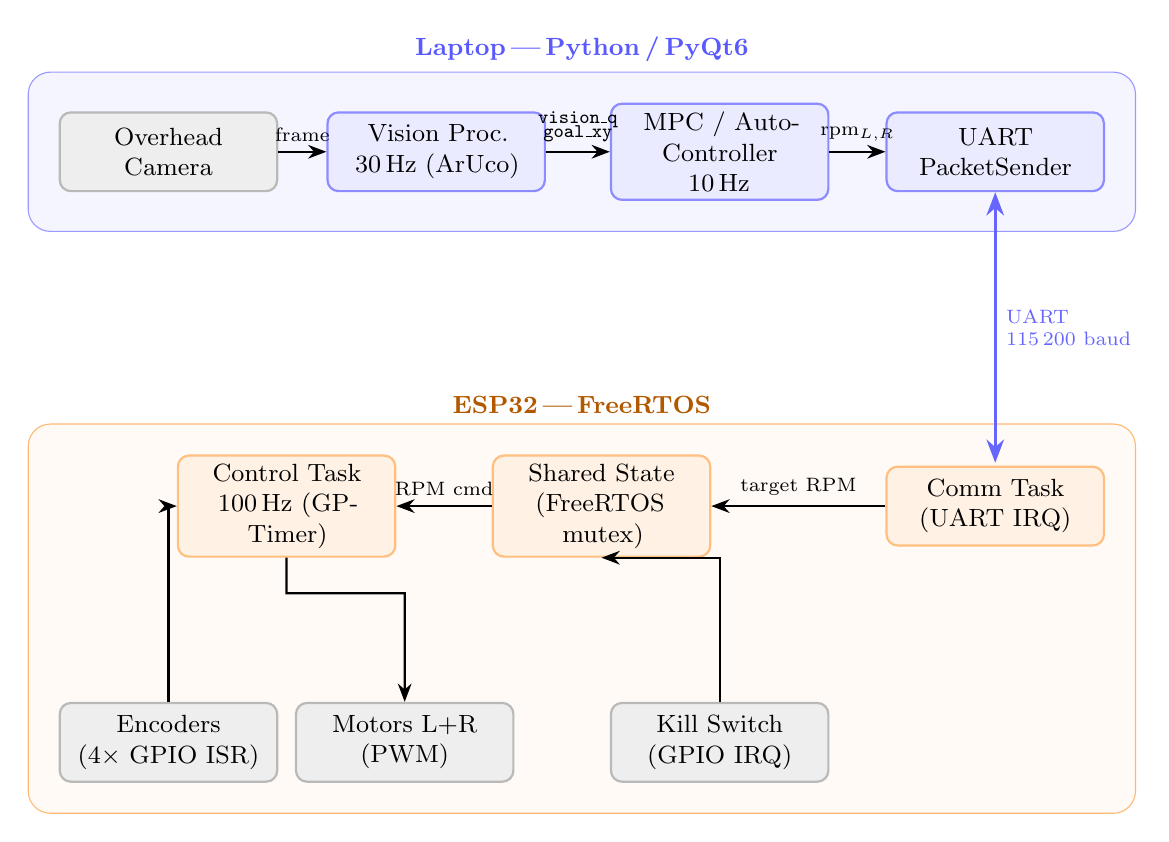
\begin{tikzpicture}[
  >=Stealth, font=\small,
  B/.style={draw, rectangle, rounded corners=4pt, thick,
            minimum height=1.0cm, text centered,
            text width=2.55cm, inner sep=3pt},
  Bl/.style={B, fill=blue!8,   draw=blue!45},
  Bo/.style={B, fill=orange!10, draw=orange!50},
  Bg/.style={B, fill=gray!13,  draw=gray!55},
  arr/.style={->, thick, >=Stealth},
  biarr/.style={<->, very thick, >=Stealth, blue!60},
]

%% ---- Laptop row (y = 0) ----
\node[Bg] (cam)  at ( 0.0, 0)  {Overhead\\Camera};
\node[Bl] (vis)  at ( 3.4, 0)  {Vision Proc.\\30\,Hz (ArUco)};
\node[Bl] (mpc)  at ( 7.0, 0)  {MPC / Auto-\\Controller\\10\,Hz};
\node[Bl] (up)   at (10.5, 0)  {UART\\PacketSender};

\draw[arr] (cam) -- node[above,font=\scriptsize]{frame} (vis);
\draw[arr] (vis) -- node[above,font=\scriptsize,align=center]
  {\texttt{vision\_q}\\[-3pt]\texttt{goal\_xy}} (mpc);
\draw[arr] (mpc) -- node[above,font=\scriptsize]{rpm$_{L,R}$} (up);

%% ---- UART vertical link ----
\draw[biarr] (up.south)
  -- node[right, font=\scriptsize, align=left]{UART\\115\,200 baud}
  (10.5,-3.95);   % top of comm.north

%% ---- ESP32 FW row (y = -4.5) ----
\node[Bo] (ct)  at ( 1.5,-4.5) {Control Task\\100\,Hz (GPTimer)};
\node[Bo] (sh)  at ( 5.5,-4.5) {Shared State\\(FreeRTOS mutex)};
\node[Bo] (cmt) at (10.5,-4.5) {Comm Task\\(UART IRQ)};

\draw[arr] (cmt) -- node[above,font=\scriptsize]{target RPM} (sh);
\draw[arr] (sh)  -- node[above,font=\scriptsize]{RPM cmd}    (ct);

%% ---- Hardware row (y = -7.5) ----
\node[Bg] (enc) at ( 0.0,-7.5) {Encoders\\(4$\times$ GPIO ISR)};
\node[Bg] (mot) at ( 3.0,-7.5) {Motors L+R\\(PWM)};
\node[Bg] (ks)  at ( 7.0,-7.5) {Kill Switch\\(GPIO IRQ)};

% enc -> ctrl  (vertical then horizontal via |- )
\draw[arr] (enc.north) |- (ct.west);
% ctrl -> motors  (down then right)
\draw[arr] (ct.south) -- ++(0,-0.45) -- ++(1.5,0) -- (mot.north);
% kill switch -> shared state
\draw[arr] (ks.north) |- (sh.south);

%% ---- Bounding boxes ----
\begin{scope}[on background layer]
  \node[draw=blue!40, fill=blue!4, rounded corners=8pt,
        fit=(cam)(vis)(mpc)(up), inner sep=11pt,
        label={[font=\small\bfseries, blue!65]above:%
               Laptop\,---\,Python\,/\,PyQt6}] {};
  \node[draw=orange!55, fill=orange!4, rounded corners=8pt,
        fit=(ct)(sh)(cmt)(enc)(mot)(ks), inner sep=11pt,
        label={[font=\small\bfseries, orange!70!black]above:%
               ESP32\,---\,FreeRTOS}] {};
\end{scope}

\end{tikzpicture}
\caption{System architecture: data flow between the laptop and ESP32.
  Solid arrows show data flow; the double-headed arrow is the
  bidirectional UART link.}
\label{fig:arch}
\end{figure}

% ---- 3. Highlights ----------------------------------------------------
\section{Highlight: Impressive Parts of the Code}

\subsection{Quadrature Encoder ISR}

In order to read the encoders using interrupts, each encoder maintains
its last 2-bit state. We use a 16-entry transition table that maps the
concatenated old and new state (a 4-bit index) to either $-1$, 0, or
$+1$ counts. An ISR fires on both the A and B edges, updates the state
only on valid transitions, and accumulates counts using an atomic
add --- safe from any concurrent context.

\begin{lstlisting}[style=clang]
static const int8_t transition_table[16] = {
    0, +1, -1, 0, -1, 0, 0, +1, +1, 0, 0, -1, 0, -1, +1, 0,
};

static void IRAM_ATTR encoder_gpio_isr(void *arg) {
  EncoderState *e = (EncoderState *)arg;
  const int a = gpio_get_level(e->pin_a);
  const int b = gpio_get_level(e->pin_b);

  const uint8_t new_state = (((a & 1) << 1) | (b & 1));
  const uint8_t index     = ((e->last_state << 2) | new_state);

  const int8_t step = transition_table[index];
  if (step != 0) {
    e->last_state = new_state;
    atomic_fetch_add(&e->pending, step);
  }
}
\end{lstlisting}

\subsection{Control Timer}

Motor control runs on a fixed period of 10\,ms (100\,Hz). A GPTimer
auto-reloads at that interval; its alarm callback calls
\texttt{vTaskNotifyGiveFromISR} to unblock the Control Task. The task
blocks on \texttt{ulTaskNotifyTake}, then runs PID, reads
targets/encoders, updates PWM, and sends telemetry. This
notify-from-ISR pattern keeps the ISR itself minimal (no computation in
interrupt context) while guaranteeing the task wakes at exactly the
right time.

\begin{lstlisting}[style=clang]
static bool IRAM_ATTR on_control_timer_alarm(
    gptimer_handle_t timer,
    const gptimer_alarm_event_data_t *edata,
    void *user_ctx) {

  TaskHandle_t control_task_handle = (TaskHandle_t)user_ctx;
  BaseType_t higher_priority_task_woken = pdFALSE;
  vTaskNotifyGiveFromISR(control_task_handle,
                         &higher_priority_task_woken);
  return higher_priority_task_woken == pdTRUE;
}
\end{lstlisting}

\subsection{MPC}

The high-level path planner is a nonlinear model predictive controller
(NMPC) implemented in Pyomo~\cite{pyomo} and solved with
IPOPT~\cite{ipopt}. At each decision step it optimizes a finite horizon
of future motion. The state vector is:
\[
  \mathbf{x} = [x,\; y,\; \theta_t,\; \theta_l,\; v,\; \omega]^\top
\]
where $(x,y)$ is the truck rear-axle position, $\theta_t$ and
$\theta_l$ are the truck and trailer headings, and $v$ and $\omega$ are
linear and angular velocity. The control inputs are linear acceleration
$a$ and angular acceleration $\alpha$.

The dynamics constraints are a discrete-time Euler integration of the
truck--trailer equations: the truck advances along its heading, headings
integrate from angular velocity, the trailer heading evolves from the
hitch geometry, and velocities integrate from the accelerations.

The optimization enforces hard limits on linear speed and turn rate, and
a jackknife constraint that keeps the heading difference
$|\theta_t - \theta_l| \leq \theta_{\max}$ so the configuration stays
physically plausible.

The objective is a weighted sum of squared errors: it penalizes missing
the desired pose at the end of the horizon, missing the goal at
intermediate steps, and using too much control effort.

\begin{lstlisting}[style=python]
def _build_model(self) -> pyo.ConcreteModel:
    c = self.cfg
    m = pyo.ConcreteModel()
    m.T     = pyo.RangeSet(0, c.N)
    m.K     = pyo.RangeSet(0, c.N - 1)
    m.S     = pyo.RangeSet(0, 5)
    m.x     = pyo.Var(m.S, m.T, domain=pyo.Reals)
    m.a     = pyo.Var(m.K, bounds=(c.a_min,     c.a_max))
    m.alpha = pyo.Var(m.K, bounds=(c.alpha_min, c.alpha_max))

    def dyn_rule(model: Any, s: int, k: int):
        if s == 0:
            return (model.x[0, k+1] ==
                    model.x[0, k] + c.dt*model.x[4, k]*pyo.cos(model.x[2, k]))
        if s == 1:
            return (model.x[1, k+1] ==
                    model.x[1, k] + c.dt*model.x[4, k]*pyo.sin(model.x[2, k]))
        if s == 2:
            return (model.x[2, k+1] ==
                    model.x[2, k] + c.dt*model.x[5, k])
        if s == 3:
            return (model.x[3, k+1] ==
                    model.x[3, k] + c.dt*(model.x[4, k]/c.d)
                    *pyo.sin(model.x[2, k] - model.x[3, k]))
        if s == 4:
            return (model.x[4, k+1] ==
                    model.x[4, k] + c.dt*model.a[k])
        if s == 5:
            return (model.x[5, k+1] ==
                    model.x[5, k] + c.dt*model.alpha[k])

    m.dyn = pyo.Constraint(m.S, m.K, rule=dyn_rule)
    m.vel_bounds = pyo.Constraint(
        m.T, rule=lambda model, t:
        pyo.inequality(c.v_min, model.x[4, t], c.v_max))
    m.omega_bounds = pyo.Constraint(
        m.T, rule=lambda model, t:
        pyo.inequality(c.omega_min, model.x[5, t], c.omega_max))
    m.jackknife = pyo.Constraint(
        m.T, rule=lambda model, t:
        pyo.inequality(-c.max_jackknife_angle,
                       model.x[2, t] - model.x[3, t],
                       c.max_jackknife_angle))

    def obj_rule(model: Any):
        cost = (
            c.w_pos * ((model.x[0, c.N] - c.q_des[0])**2
                     + (model.x[1, c.N] - c.q_des[1])**2)
            + c.w_theta_t * (model.x[2, c.N] - c.q_des[2])**2
            + c.w_theta_l * (model.x[3, c.N] - c.q_des[3])**2
            + c.w_v       * (model.x[4, c.N] - c.q_des[4])**2
            + c.w_omega   * (model.x[5, c.N] - c.q_des[5])**2
        )
        cost += sum(
            c.w_pos_stage
            * ((model.x[0, k] - c.q_des[0])**2
             + (model.x[1, k] - c.q_des[1])**2)
            for k in range(c.N)
        )
        cost += sum(
            c.w_a * model.a[k]**2 + c.w_alpha * model.alpha[k]**2
            for k in range(c.N)
        )
        return cost

    m.obj = pyo.Objective(rule=obj_rule, sense=pyo.minimize)
    return m
\end{lstlisting}

% ---- 4. Time Machine --------------------------------------------------
\section{Time Machine --- What We Would Do Differently}

If we could go back to the start of the project, we would do most of
what we did over again. However, there are some improvements that would
have been nice to add, and things we would do differently.

\subsection{Hardware Jackknife Detection}

Right now the jackknife constraint only lives in the MPC optimization
and relies entirely on the vision-based state estimate. We do have a
sensor on the hitch angle (the potentiometer), but its accuracy is lower
than the vision-derived estimate due to the quality of the
potentiometer. If we could go back, we would source a higher-quality
angle sensor. This would allow us to use the hitch angle directly in the
MPC instead of relying on the camera, and would also enable a hardware
interrupt on the ESP32 that cuts motor power immediately if a jackknife
condition is detected --- faster and more reliable than waiting for the
next MPC iteration.

\subsection{Obstacle-Aware MPC}

The current MPC has no awareness of obstacles other than the jackknife
angle. In a real parking scenario the truck would need to avoid walls
and other objects. An improvement would be to add obstacle constraints
to the MPC formulation. The camera already has a full overhead view of
the scene, so obstacle detection is feasible with the existing vision
setup; however, this would increase the complexity and solve time of the
MPC.

\subsection{Parallel-Parking MPC}

The current MPC drives the truck to park into a pre-determined spot
regardless of the relative angles. In a real parking scenario the truck
would want to park in parallel --- that is, with the trailer aligned to
the parking space at a specified heading. An improvement would be to add
an additional angle state (trailer-to-parking-spot heading error) to the
MPC state vector. The CV already detects all ArUco markers including the
parking spot, so adding one more state is feasible with the existing
vision setup; however, this would require changing cost functions and
would potentially increase MPC complexity and solve time.

% ---- 5. Conclusion ----------------------------------------------------
\section{Conclusion}

This project demonstrated a full-stack embedded control system for
autonomous truck-trailer reverse parking. On the hardware side, an ESP32
running FreeRTOS achieved hard real-time motor control at 100\,Hz using
a GPTimer ISR, quadrature encoder interrupts, dual independent PID
loops, and FreeRTOS mutex-protected shared state between the Control and
Communication tasks. On the software side, a laptop-hosted Python stack
combined an overhead ArUco vision pipeline (30\,Hz), a nonlinear MPC
planner (10\,Hz, Pyomo/IPOPT), and a PyQt6 GUI into a single
event-driven application. The system successfully performed closed-loop
autonomous parking maneuvers on the physical model, with the MPC
enforcing the jackknife constraint throughout the trajectory.

Building an embedded system that spans hardware, software, real-time
control, computer vision, nonlinear optimization, and a GUI was a fun,
challenging, and rewarding project.

% ---- References -------------------------------------------------------
\begin{thebibliography}{9}

\bibitem{freertos}
  FreeRTOS.org.
  \textit{FreeRTOS Kernel Developer Documentation}.
  \url{https://www.freertos.org/Documentation/RTOS_book.html}

\bibitem{pyomo}
  W.\,E.~Hart, C.\,D.~Laird, J.-P.~Watson, D.\,L.~Woodruff,
  G.\,A.~Hackebeil, B.\,L.~Nicholson, and J.\,D.~Siirola.
  \textit{Pyomo --- Optimization Modeling in Python}, 2nd~ed.
  Springer, 2017.

\bibitem{ipopt}
  A.~W\"{a}chter and L.\,T.~Biegler.
  On the implementation of an interior-point filter line-search
  algorithm for large-scale nonlinear programming.
  \textit{Mathematical Programming}, 106(1):25--57, 2006.

\bibitem{aruco}
  S.~Garrido-Jurado, R.~Mu\~{n}oz-Salinas, F.\,J.~Madrid-Cuevas,
  and M.\,J.~Mar\'{\i}n-Jim\'{e}nez.
  Automatic generation and detection of highly reliable fiducial
  markers under occlusion.
  \textit{Pattern Recognition}, 47(6):2280--2292, 2014.

\bibitem{truck_trailer}
  J.-P.~Laumond, P.~Jacobs, M.~Ta\"{\i}x, and R.~Murray.
  A motion planner for nonholonomic mobile robots.
  \textit{IEEE Trans.\ Robotics and Automation}, 10(5):577--593, 1994.

\end{thebibliography}

\end{document}
